\documentclass[12pt]{article}
\usepackage{amsmath}
\usepackage[rm,tiny,explicit]{titlesec}
\usepackage[margin=1in]{geometry}
\usepackage{subfigure}
\usepackage[subfigure]{tocloft}
\usepackage{etoolbox}
\usepackage{graphicx}
\usepackage{chngcntr}
\usepackage{afterpage}
\usepackage{pdfpages}
\usepackage{fancyvrb}
\usepackage{listings}
\usepackage[euler]{textgreek}
\counterwithin{figure}{section}
\counterwithin{table}{section}
\usepackage[labelfont=bf]{caption}
\usepackage{enumitem}
\setlist{nolistsep}
\usepackage{wasysym}
\usepackage{multirow}
\usepackage{booktabs}
\usepackage[titletoc,toc,title]{appendix}

\renewcommand\cftsecfont{\normalfont}
\renewcommand\cftsecpagefont{\normalfont}
\renewcommand{\cftsecleader}{\cftdotfill{\cftdotsep}}

%Add table padding
\renewcommand{\arraystretch}{1.25} % Default value: 1

\titleformat{\section}{\normalfont\centering\bfseries}{\thesection}{1em}{\MakeUppercase{#1}}
\titleformat{\subsection}{\normalfont\flushleft\bfseries}{\thesubsection}{1em}{#1}
\titleformat{\subsubsection}{\normalfont\flushleft\bfseries}{\thesubsubsection}{1em}{#1}


\setcounter{secnumdepth}{3}
\setcounter{tocdepth}{2}

\renewcommand{\floatpagefraction}{.8}
\renewcommand{\topfraction}{.8}
\renewcommand{\textfraction}{.2}

% required by \up and \down
\usepackage{amsmath}

% add superscripts OUTSIDE of math mode
\newcommand{\up}[1]{$^\text{#1}$}

% add subscripts OUTSIDE of math mode
\newcommand{\down}[1]{$_\text{#1}$}

% remove border from cell
\newcommand{\nob}[1]{\multicolumn{1}{c}{#1}}

% Duct tape Appendix
\newcommand{\app}[2][\null]{
	\clearpage
 	\newpage
 	{
 	 	\centering
 	 	\addcontentsline{toc}{section}{Appendix #2}
% 	 	\textbf{APPENDIX A} \\ \bigskip
		\section*{APPENDIX #2}
 	 	\textbf{#1} \\ \bigskip
 		}
}
\graphicspath{{img/}}

\begin{document}  	
	\addcontentsline{toc}{section}{Title Page}
	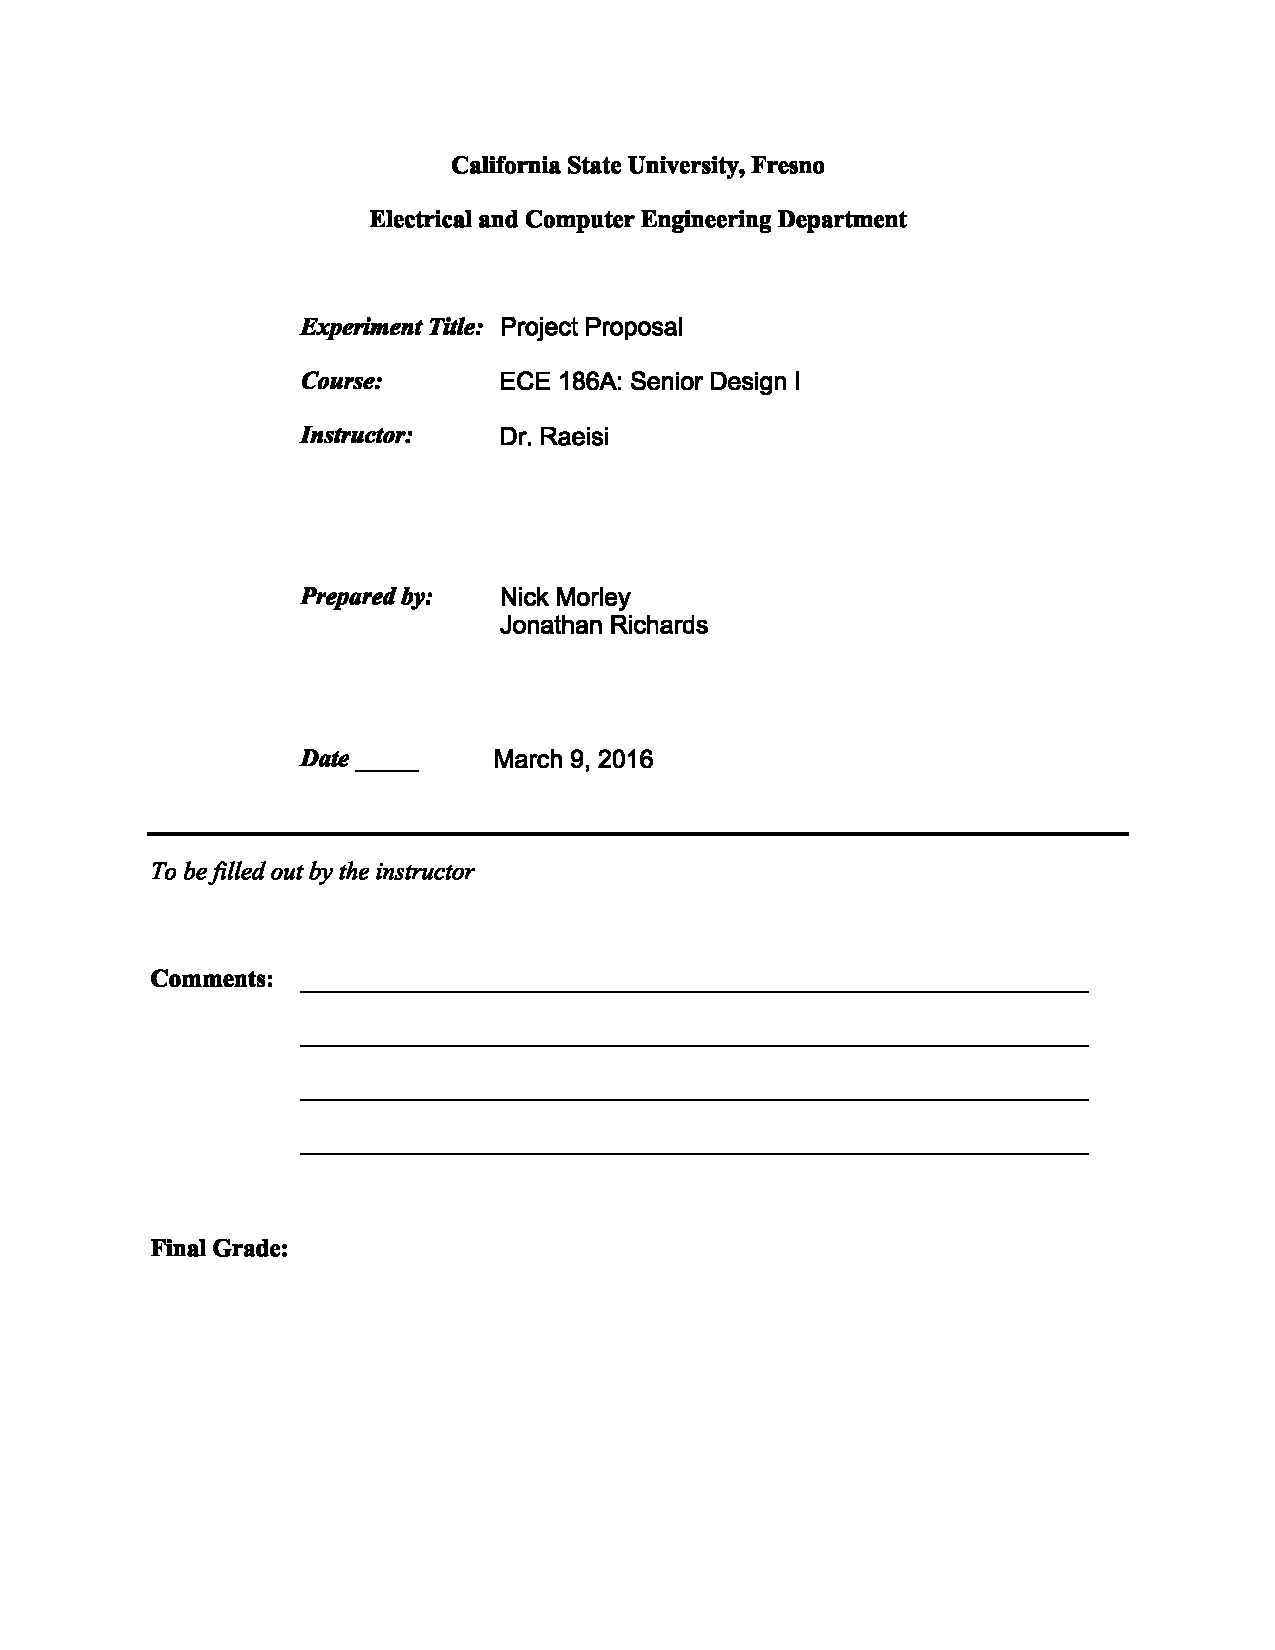
\includepdf[pages=1]{cover.pdf}
	\renewcommand*\contentsname{
		\begin{align*}
			\normalsize \textbf{TABLE OF CONTENTS}
		\end{align*}
		\noindent\makebox[\textwidth]{\normalsize \textbf{Section}\hfill \normalsize  \textbf{Page}}
	}
	\addcontentsline{toc}{section}{Table of Contents}  	
	\tableofcontents
	
	\newpage
	
	\section{The Team}
		\vfill
		\begin{tabular}{l l}
			Team Name:    & Sensor Network    \\
			\\
			Team Members: & Nick Morley       \\
			              & Jonathan Richards \\
%			              & Daniel Kline\\
			              \\
			Technical Advisor: & Dr. Hovannes Kulhandjian\\
			\\
			Course Instructor: & Dr. Reza Raeisi\\
		\end{tabular}
		 
	\section{Goals}
		\begin{itemize}
			\item Create a system to collect, transport, analyze, store, and visualize sensor data
			\item Control external systems manually or automatically according to sensor inputs
			\item Access user interface anywhere with an internet connection
		\end{itemize}
		
	\section{Objectives}
		\subsection{Modularity}
			\begin{itemize}
				\item The network shall be modular and be composed of a wireless network of similar nodes with one base station
				\item The nodes shall be modular and support a variety of sensors and controllers interfacing over a common hardware/software interface
			\end{itemize}
			
		\subsection{Dynamic}
			\begin{itemize}
				\item The network shall be able to respond to the dynamic addition or removal of nodes
				\item The nodes shall support hot-plugging of sensors
				\item The client application shall view live data from the sensors
			\end{itemize}
			
		\subsection{Interactive}
			\begin{itemize}
				\item The nodes shall generate alerts for the user to respond to
				\item The user shall control the node's sensors and controllers from the client application
			\end{itemize}
		\subsection{Easy to Use}
			\begin{itemize}
				\item The user application shall allow easy configuration of new nodes and sensors
				\item The historic data shall be presented in a clean, graphical manner to the user
				\item The user interface shall be intuitive and user friendly
			\end{itemize}
			
	\section{Background}
		\subsection{Microcontroller Programming and Interfacing}
			Both team members of our team have experience programming a wide variety of microcontrollers to interface with the outside world. This knowledge will be vital to interfacing with the sensors to gather data into our network and controlling exterior devices. It will also be useful for interprocessor communication to relay messages from one end of the network to the other (including the user's phone).
		
		\subsection{Wireless Communication}
			Nick has some experience with establishing communication between a few processors through multiple point to point links. This will help us get starting, but we will put further research into how to implement a mesh network, including routing algorithms.
		
		\subsection{Data Storage, Processing, and Serving}
			Both team members have some server-side experience in spinning up servers and presenting data to the user from a database. Nick also has experience funneling data into the database that will be important for establishing communication between the server and base station to transfer data into the database. Since our sensor data will be highly compressable, we will implement a custom compression algorithm to minimize network and server resources.
			
		\subsection{Mobile App Development}
			Both team members have some web application experience we will leverage for first creating a web interface to our network. We will then port our web application to Android and iOS.
 
	 \section{Feasibility}
		 \subsection{ESP8266 Microcontroller}
			 The ESP8266 microcontroller is a low cost microcontroller with integrated, long-range wireless communications that will be the master control unit of each node. The most important features for our purposes are:
			 \begin{itemize}
			 	\item Unit cost of \$2.44 in lots of 10 or more
			 	\item Range of 366 meters with standard consumer wireless router and range of 3.71 kilometer with long range access point
			 	\item I$^2$C interface for communicating with sensor modules
			 	\item Analog to digital converter for monitoring supply voltage (if we deploy battery powered nodes)
			 	\item UART port (if we interface multiple ESP8266s on a node)
			 	\item 13 general purpose input/output pins for buttons and status LEDs
			 \end{itemize}
			 
		\subsection{ATmega328P Microcontroller}
			The ATmega328P microcontroller is a low cost, general purpose microcontroller. To simplify the software and hardware interface between the sensors and our network, each sensor module will contain an ATmega328P. This enables a simple, common interface between the node and sensor module over I$^2$C and offloads the sensor monitoring from the ESP8266. It also makes the sensor modules more universal since adding or changing sensors will not require a firmware update on the node itself. Instead the sensor specific firmware is stored on the ATmega328P that is bundled with the sensor. The most important features for our purposes are:
			\begin{itemize}
				\item Unit cost of \$1.21 in lots of 10 or more
				\item Wide variety of intefaces to talk to the sensor based on it's specific needs
				\begin{itemize}
					\item 20 genneral purpose input/output pins
					\item 8 channel analog to digital converter
					\item 6 pulse width modulation outputs
					\item SPI
					\item UART
					\item I$^2$C
					\item OneWire
				\end{itemize}
			\end{itemize}
		
		\subsection{2.8'' TFT LCD Touchscreen}
		The touchscreen allows the node to have a direct and convienent user interface. For example, on a thermostat it would allow the user to see the current temperature, change the set point, view the energy usage of the air conditioner, and view a plot of the temperature without having to pull up the client app. It can also be used to aid in the initial setup process. It is not strictly necessary, but offers a polished feel to the system for the user to immediately see the system working. The most important features for our purposes are:
		\begin{itemize}
			\item Unit cost of \$8.19
			\item Full color screen for displaying user interface
			\item Touch enabled for user input
		\end{itemize}
		
		\subsection{DHT22 Sensor}
			The DHT22 temperature and humidity sensor can serve for either a weather station or thermostat node. It interfaces with the ATmega328P over a digital bus. The most important features for our purposes are:
			\begin{itemize}
				\item Unit cost of \$5.99
				\item Temperature range of -40 - 80 $^\circ$C
				\item Temperature accuracy of $\pm$ 0.5 $^\circ$C
				\item Humidity range of 0 - 100\% RH
				\item Humidity accuracy of $\pm$ 2\% RH
			\end{itemize}
		
		\subsection{AC Current Sensor}
			The current sensor is non-invasive and plugs into a 3.5 mm TRS connector. Since it is non-invasive, the client safely clips it around the device they would like to measure without having to cut any wires. The most important features for our purposes are:
			\begin{itemize}
				\item Unit cost of \$11.19
				\item Measures up to 100 A loads (can be used for air conditioners or entire house)
				\item Common connector
			\end{itemize}
		
		\subsection{Barometric Pressure Sensor}
			The barometeric pressure sensor allows us to enhance a weather station's measurements or track the node's elevation. The most important features for out purposes are:
			\begin{itemize}
				\item Unit cost of \$4.34
				\item Pressure range of 300 - 1100 hPa
				\item Pressure accuracy of 0.02 hPa
				\item Elevation range of -500 - 9000 meters
				\item Elevation accuracy of 17 cm
				\item I$^2$C interface
			\end{itemize}
		
		\subsection{Brightness Sensor}
			The brightness sensor is a photoresistor that can detect the ambient brightness level of the room. It can be used to monitor when people leave the lights on or track sunrise/sunset. We can also mount multiple sensors on each module pointed in different directions The most important features for our purposes are:
			\begin{itemize}
				\item Unit cost of \$0.03 in lots of 100 or more
			\end{itemize}
		
		\subsection{Audio Sensor}
			The audio sensor is a microphone that can detect people talking or serve as a spectrum analyzer using digital signal processing. %TODO: fill in Jon
		
		% TODO: add rain, wind sensors
		
		\subsection{Cloud Server}
			The cloud server will store historic sensor data and serve the web application for the users in addition to hosting the project management software for this project. It is the single entry point for users to access the sensor network from the internet.
	 
	\section{Protocols}
		\subsection{Intranode Protocol}
			The Intranode Protocol is used to gather sensor data from the sensor and controller modules to the node. The physical layer diagramed in Figure~\ref{fig:IntranodePhysical} depicts pins connecting the systems. The link layer is composed of 32 byte packets exchanged between the systems as described in Table~\ref{tab:IntranodeLink}. All words are stored in little-endian format.
			\begin{table}[h!]
				\centering
				\caption{Intranode Packets}
				\label{tab:IntranodeLink}
				\begin{tabular}{l c c l}
					\toprule[1.2pt]
					Field Name & Byte Index & Field Width & Field Explation\\ \hline
					Address & 0 & 8 bits & Which port the sensor is plugged into\\
					Message Type & 1:2 & 16 bits & An identifier for how the payload is formated\\
					Sensor Type & 3:4 & 16 bits & An identifier for the physical sensor board\\
					Reserved & 5:6 & 16 bits & Reserved for later revisions\\
					Payload & 7:30 & 24 bytes & Message data\\
					Checksum & 31 & 8 bits & Checksum of first 31 bytes of packet\\ \bottomrule[1.2pt]
				\end{tabular}
			\end{table}
			
			\begin{figure}[h!]
				\centering
				\includegraphics[width=\textwidth, angle=0]{IntranodeProtocol}
				\caption{The connections between the node and sensor module}
				\label{fig:IntranodePhysical}
			\end{figure}
	
		\subsection{Touchscreen Protocol}
			The touchscreen communicates with the ATmega328P over a bi-directional parallel port according to the five status bits as diagrammed in Figure~\ref{fig:TFTProtocol} and Table~\ref{tab:TouchscreenProtocol}. To write data to the LCD, the ATmega328P brings CS low to enable the touchscreen. It then asserts CD low for sending a command or high for sending data followed by placing the data to transmit on the data bus. Finally, the ATmega329P brings WR low for a few clock cycles and back high. To read data from the LCD, the ATmega328P brings CS low to enable the touchscreen, brings RD low for a few clock cycles, and brings RD back high. It then reads the byte off the data bus.
			\begin{table}[h!]
				\centering
				\caption{Touchscreen Physical Interface}
				\label{tab:TouchscreenProtocol}
				\begin{tabular}{c c l}
					\toprule[1.2pt]
					Pin Symbol & Pin Name & Pin Explation\\ \hline
					$\overline{\textrm{CS}}$ & $\overline{\textrm{Chip Select}}$ & Enables touchscreen communications when low\\
					CD & $\overline{\textrm{Command}}$/Data & 0: Command, 1: Data\\
					WR & Write & Writes data to the touchscreen on falling edge\\
					RD & Read & Reads data from the touchscreen on falling edge\\
					$\overline{\textrm{RST}}$ & $\overline{\textrm{Reset}}$ & Resets the touchscreen when low\\
					D7:D0 & LCD Data & A byte transmitted between ATmega328P and touchscreen\\ \bottomrule[1.2pt]
				\end{tabular}
			\end{table}
			
			\begin{figure}[h!]
				\centering
				\includegraphics[width=\textwidth, angle=0]{TFTProtocol}
				\caption{The connections between the touchscreen and ATmega328P}
				\label{fig:TFTProtocol}
			\end{figure}
			
	
		\subsection{DHT22 Protocol}
			The DHT22 communicates over a digital, bi-directional, single pin bus that is normally high through the connections made in Figure~\ref{fig:DHT22Protocol}. To begin a transmition, the ATmega first brings the bus low for at least 1 ms by configuring the pin as a digital output with a value of zero. It then configures the pin as a digital input with a weak pullup. 40 \textmu s later, the DHT22 brings the bus low for 80 \textmu s and high for 80 \textmu s to indicate that it is about to begin transmission as shown in Figure~\ref{fig:DHT22init}. The DHT22 then brings the bus low for 50 \textmu s and high for a variable amount of time. If the bus is high for 26 - 28 \textmu s, the bit is interpretted as a ``0'' as shown in Figure~\ref{fig:DHT22low}. If the bus is high for 70 \textmu s, the bit is interpretted as a ``1'' as shown in Figure~\ref{fig:DHT22high}. After all 40 bits have been transmitted, the DHT22 lets the bus float high. Note that the highest bit is transmitted first.
			
			\begin{figure}[h!]
				\centering
				\includegraphics[width=\textwidth, angle=0]{DHT22Protocol}
				\caption{The connections between the sensor module and DHT22}
				\label{fig:DHT22Protocol}
			\end{figure}
			
			\begin{figure}[h!]
				\centering
				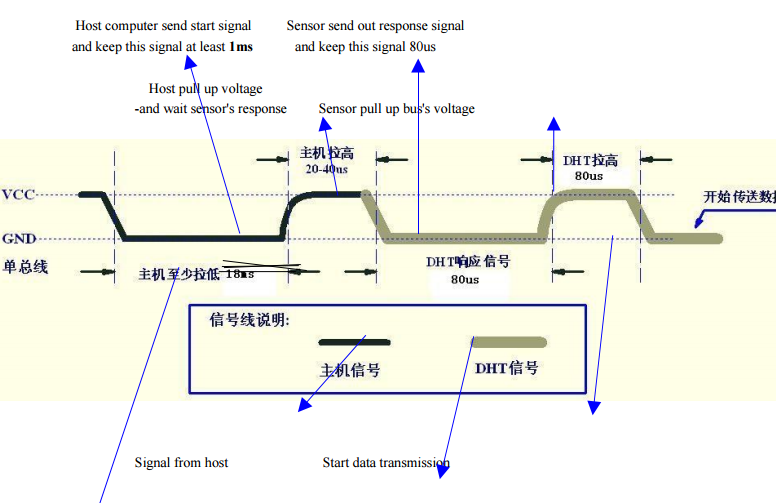
\includegraphics[width=\textwidth, angle=0]{DHT22init}
				\caption{The initialization of a reading between the ATmega328P and DHT22}
				\label{fig:DHT22init}
			\end{figure}
			
			\begin{figure}[h!]
				\centering
				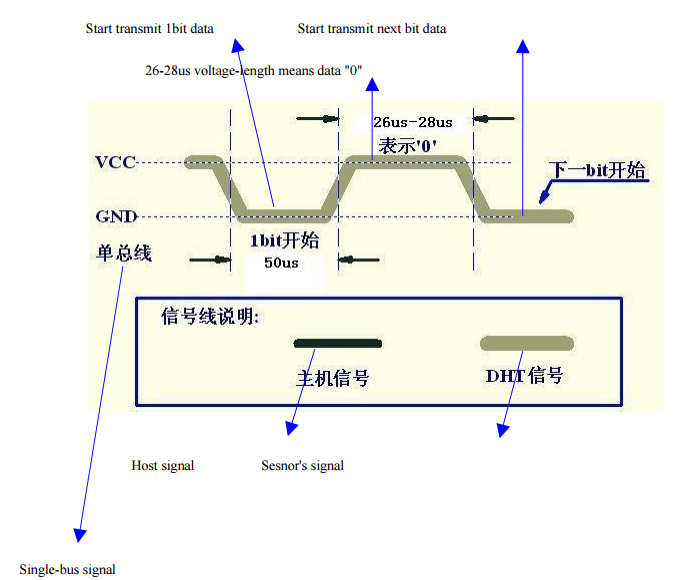
\includegraphics[width=\textwidth, angle=0]{DHT22low}
				\caption{The DHT22 trasnmitting a ``0''}
				\label{fig:DHT22low}
			\end{figure}
			
			\begin{figure}[h!]
				\centering
				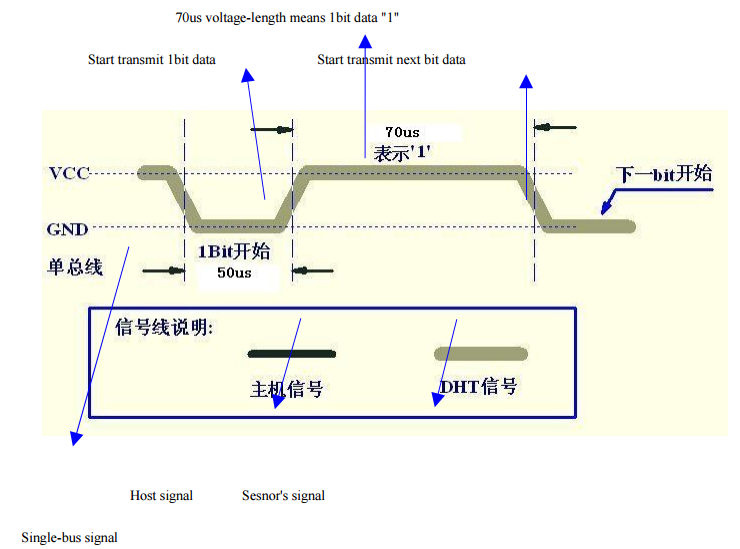
\includegraphics[width=\textwidth, angle=0]{DHT22high}
				\caption{The DHT22 transmitting a ``1''}
				\label{fig:DHT22high}
			\end{figure}
			
			\clearpage
			
		\subsection{AC Current Sensor}
			The current sensor uses a transformer to induce a current between 0 and 50 mA (RMS) at 60 Hz on the secondary coil. This current is passed through the RC network in Figure~\ref{fig:CurrentSensorProtocol} to generate a sinisoid centered at 2.5 V oscilating between 0 V and 5 V. This wave is sampled on the ATmega328P's analog input channel to calculate the RMS current though the primary coil. With the 10 bit ADC on the ATmega328P, this translates to a 98 mA (RMS) resolution on the primary coil's current.
				\begin{figure}[h!]
					\centering
					\includegraphics[width=\textwidth, angle=0]{CurrentSensorProtocol}
					\caption{The connections between the sensor module and current sensor}
					\label{fig:CurrentSensorProtocol}
				\end{figure}
		
		
		\subsection{Barometric Pressure Sensor}
			The barometric pressure sensor communicates with the ATmega328P through an I$^2$C bus as depicted in Figure~\ref{fig:BMP180protocol}. It does this by triggering the BMP180, reading the calibration data, reading the raw pressure reading, and calculating the true pressure data according to Figure~\ref{fig:BMP180flowchart}. The calibration and status register addresses are recored in Figures~\ref{fig:BMP180calibration}~and~\ref{fig:BMP180registers}, respectively. Once the barometric pressure has been calculated, the ATmega328P calculates the altitude from the relationship in Figure~\ref{fig:BMP180altitude}.
			
			\begin{figure}[h!]
				\centering
				\includegraphics[width=\textwidth, angle=0]{BMP180Protocol}
				\caption{The interface between the ATmega328P and BMP180}
				\label{fig:BMP180protocol}
			\end{figure}
			
			\begin{figure}[h!]
				\centering
				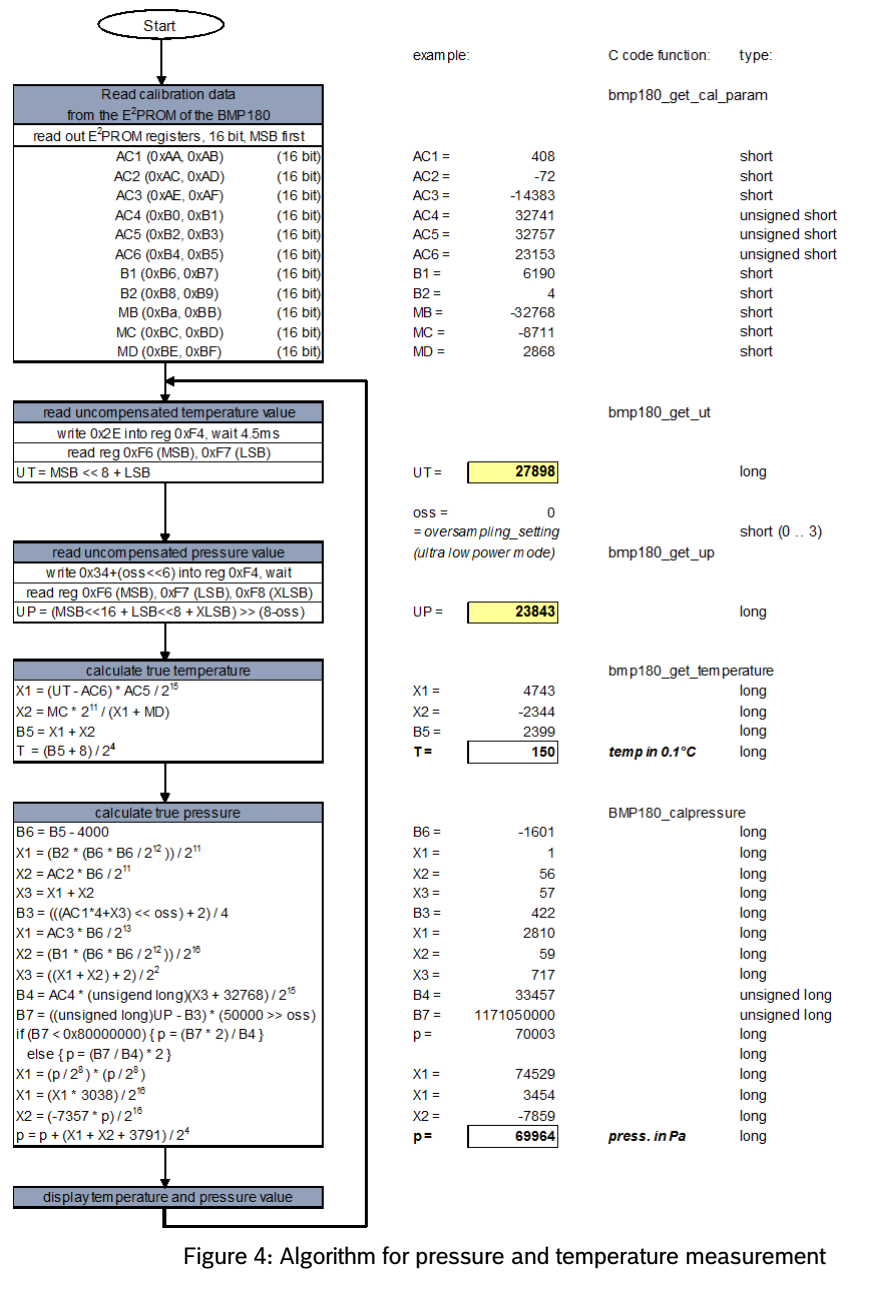
\includegraphics[height=0.95\textheight, angle=0]{BMP180flowchart}
				\caption{The program flow for reading the BMP180}
				\label{fig:BMP180flowchart}
			\end{figure}
			
			\begin{figure}[h!]
				\centering
				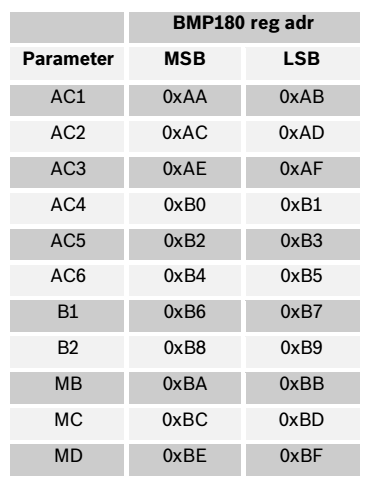
\includegraphics[width=0.4\textwidth, angle=0]{BMP180calibration}
				\caption{The calibration registers for the BMP180}
				\label{fig:BMP180calibration}
			\end{figure}
			
			\begin{figure}[h!]
				\centering
				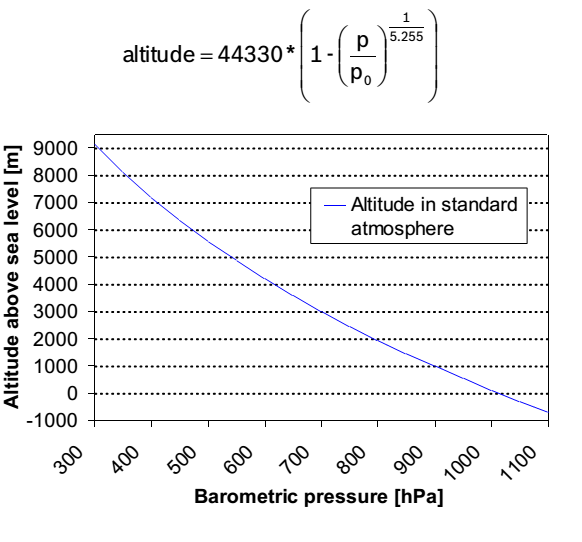
\includegraphics[width=0.6\textwidth, angle=0]{BMP180altitude}
				\caption{The relationship between barometric pressure and altitude}
				\label{fig:BMP180altitude}
			\end{figure}
			
			\begin{figure}[h!]
				\centering
				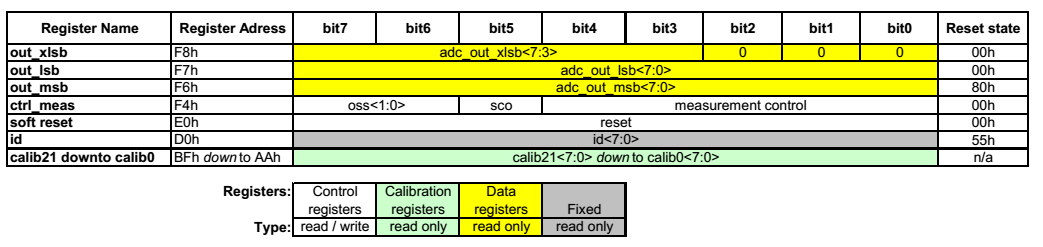
\includegraphics[width=0.95\textheight, angle=90]{BMP180registers}
				\caption{The status registers of the BMP180}
				\label{fig:BMP180registers}
			\end{figure}
			
		
			\clearpage
		
		\subsection{Brightness Sensor}
			The brightness sensors connect to the ATmega328P's ADC channels where a higher analog voltage represents a brighter room. There are six brightness sensors on each sensor module, allowing for light detection in six directions as shown in Figure~\ref{fig:BrightnessSensorProtocol}.
			
			\begin{figure}[h!]
				\centering
				\includegraphics[width=\textwidth, angle=0]{BrightnessSensorProtocol}
				\caption{The interface between the brightness sensors and ATmega328P}
				\label{fig:BrightnessSensorProtocol}
			\end{figure}
			
		\subsection{Audio Sensor}
			The audio sensor %TODO: start, add schematic, etc
		
	 \section{Input/Output Diagram}
		 The logical datapath for the project is diagramed in Figure~\ref{fig:BlockDiagram}. The network diagram for connecting different physical modules are presented in Figure~\ref{fig:NetworkDiagram}. The inputs/outputs are summarized below.
		 \begin{itemize}
		 	\item Sensor Data
		 	\begin{itemize}
		 		\item Temperature
		 		\item Humidity
%		 		\item Wind Speed
%		 		\item Rainfall
		 		\item Barometric Pressure / Elevation
		 		\item Current / Energy usage
		 		\item Brightness
		 		\item Sound
		 	\end{itemize}
		 	\item Control Devices
		 	\begin{itemize}
		 		\item Air Conditioner / Heater
		 		\item LEDs
		 		\item Outlets
		 		\item Lights
		 	\end{itemize}
		 	\item Node Configuration
		 	\begin{itemize}
		 		\item Sampling Rate
		 		\item Precision
		 		\item Control Conditions
		 		\item Network
		 		\item Link to Account
		 	\end{itemize}
		 	\item Plotted Sensor Data
		 	\begin{itemize}
		 		\item Organize sensor data graphically for user
		 	\end{itemize}
		 	\item Sensor Data Analytics
		 	\begin{itemize}
		 		\item Averages
		 		\item Cummulative Totals
		 	\end{itemize}
		 	\item Network Status
		 	\begin{itemize}
		 		\item Nodes online
		 		\item Last sensor readings
		 	\end{itemize}
		 \end{itemize}
	 
		\begin{figure}[h!]
			\centering
			\includegraphics[height=0.8\textwidth, angle=90]{BlockDiagram}
			\caption{The Logical Datapath}
			\label{fig:BlockDiagram}
		\end{figure}
		
		\clearpage
		
		\begin{figure}[h!]
			\centering
			\includegraphics[height=\textwidth, angle=90]{NetworkDiagram}
			\caption{The Physcical Datapath}
			\label{fig:NetworkDiagram}
		\end{figure}
		
		\clearpage
		 
	\section{Project Timeline}
	
		\begin{figure}[h!]
			\centering
			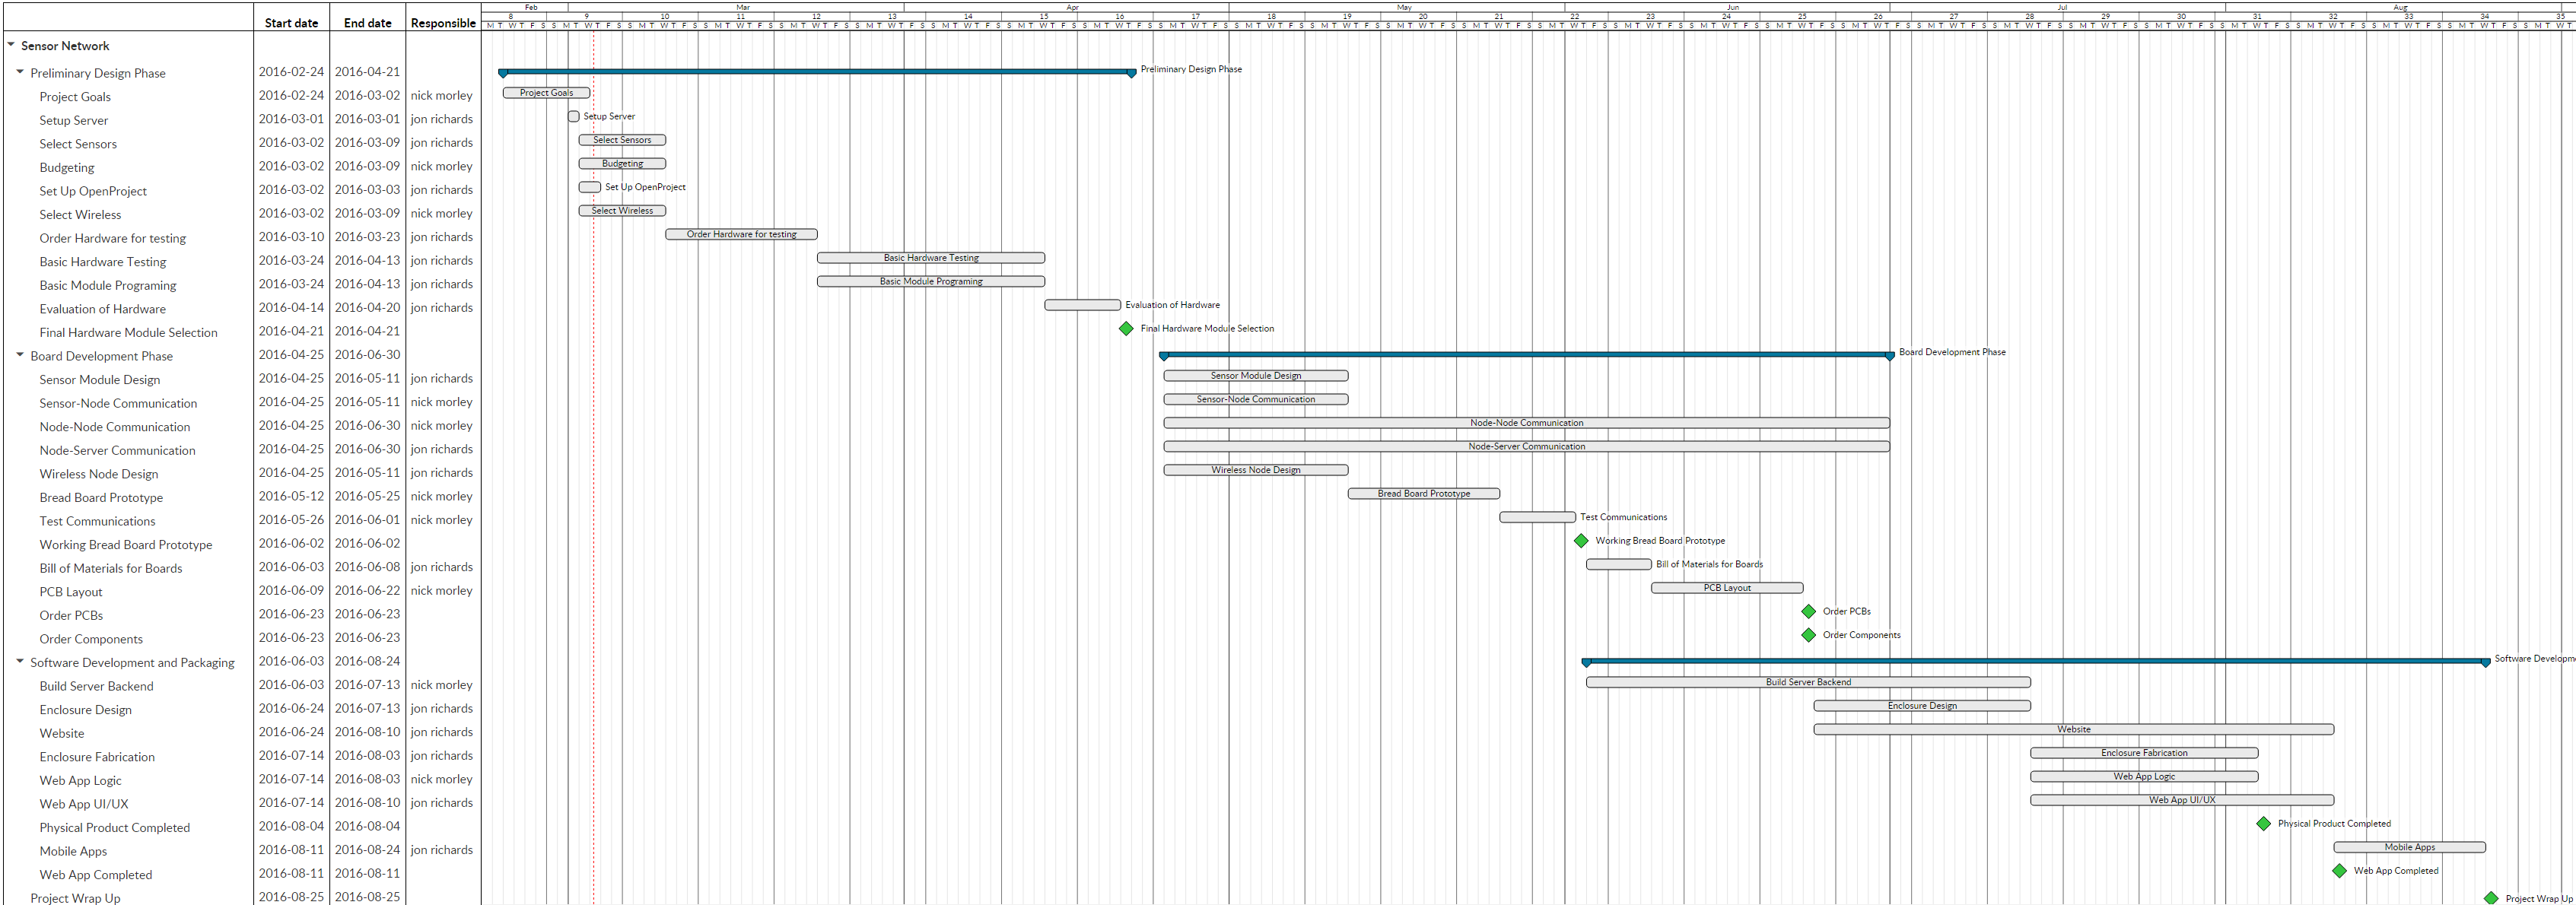
\includegraphics[width=0.85\textheight, angle=90]{GantChart}
			\caption{Gant Chart for Project Timeline}
			\label{fig:GantChart}
		\end{figure}
		 
		 
%	 \newpage
%	 \section{Approval}
%		\begin{flushleft}
%			I agree to build the above project throughout ECE 186A and 186B.\\
%			\vspace{2em}
%			\begin{tabular}{l l l}
%				\line(1,0){250} & \hfill & \line(1,0){100}\\
%				\textit{Team Member Signature} & & \textit{Date}				
%			\end{tabular}
%			\vspace{2em}\\
%			\begin{tabular}{l l l}
%				\line(1,0){250} & \hfill & \line(1,0){100}\\
%				\textit{Team Member Signature} & & \textit{Date}
%			\end{tabular}
%%			\vspace{2em}\\
%%			\begin{tabular}{l l l}
%%				\line(1,0){250} & \hfill & \line(1,0){100}\\
%%				\textit{Team Member Signature} & & \textit{Date}
%%			\end{tabular}
%			\vspace{5em}
%			
%			I agree to be the formal, technical adivsor to this project.\\
%			\vspace{2em}
%			\begin{tabular}{l l l}
%				\line(1,0){250} & \hfill & \line(1,0){100}\\
%				\textit{Technical Advisor Signature} & & \textit{Date}
%			\end{tabular}
%			\vspace{5em}
%			
%			I approve this project to be a viable capstone project.\\
%			\vspace{2em}
%			\begin{tabular}{l l l}
%				\line(1,0){250} & \hfill & \line(1,0){100}\\
%				\textit{Course Instructor Signature} & & \textit{Date}
%			\end{tabular}
%		\end{flushleft}		 
		 
\end{document}